\begin{frame}
\frametitle{The Tutte algorithm}
\framesubtitle{Synchronous VS Asynchronous}
Two approach to the Tutte algorithm :
\begin{exampleblock}{}
\begin{itemize}
\item Asynchronous : Each movement is applied directly after being computed
\item Synchronous : All movements are computed before being applied
\end{itemize}
\end{exampleblock}{}
\end{frame}

\begin{frame}[fragile]
\frametitle{The Tutte algorithm parallel}
\framesubtitle{Graph coloring}
\begin{exampleblock}{}
\begin{verbatim}
G={V,E}
Y = V
color = 0
While Y is not empty
   Z = Y
   While Z is not empty
      Choose a node v from Z
      Colorate v with color
      Y = Y - v
      Z = Z - v - {neighbors of v}
   End while
   color ++
End while
\end{verbatim}
\end{exampleblock}{}
\end{frame}

\begin{frame}
\frametitle{The Tutte algorithm parallel}
\framesubtitle{Asynchronous}
\begin{exampleblock}{}
\begin{figure}[!h]
\centering
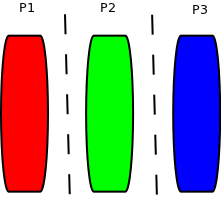
\includegraphics[scale=0.5]{../rapport/img/distribution_verticale.png}
\end{figure}
\end{exampleblock}{}
\pause
\begin{exampleblock}{}
\begin{figure}[!h]
\centering
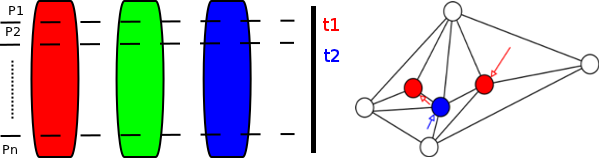
\includegraphics[scale=0.5]{../rapport/img/distrib.png}
\end{figure}
\end{exampleblock}{}
\end{frame}

\begin{frame}
\frametitle{The Tutte algorithm parallel}
\framesubtitle{Synchronous}
\begin{exampleblock}{}
\begin{figure}[!h]
\centering
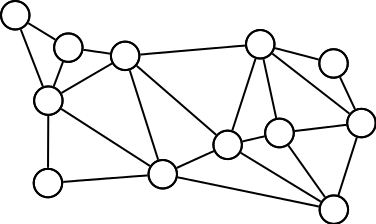
\includegraphics[scale=0.4]{../rapport/img/g12.png}
\end{figure}
\end{exampleblock}{}
\pause
\begin{exampleblock}{}
\begin{figure}[!h]
\centering
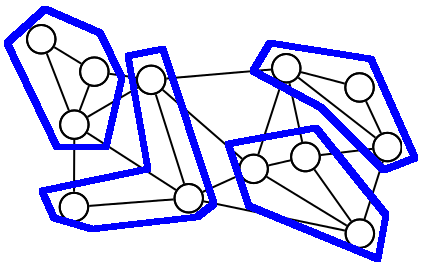
\includegraphics[scale=0.4]{../rapport/img/g12_parted.png}
\end{figure}
\end{exampleblock}{}
\end{frame}
